\appendixchapter{de Rham Cohomology}
\label{app:cohomology}
\chaptermark{de Rham Cohomology}
\section*{Introduction}
Chapter~13 proves $d^2=0$. Thus a form that is a derivative is automatically
closed. The converse question is more subtle:
\[
d\omega=0\quad\stackrel{?}{\Longrightarrow}\quad\omega=d\eta.
\]
Locally the answer is yes in positive degree. Globally a hole can prevent
local primitives from fitting together. De Rham cohomology organizes that
failure of global exactness, and integration provides a way to detect it.
Here closed means $d\omega=0$ and exact means $\omega=d\eta$;
\cref{def:de-rham-cohomology} will collect the precise quotient definition.

This appendix starts from forms, pullbacks, and Stokes in Chapter~13.
Appendix~\ref{app:quotients} enriches its geometric examples, while
Appendices~\ref{app:submanifolds} and~\ref{app:lie} are not prerequisites.
Compare Tu~\cite[\S\S24--29]{tu-manifolds} and
Lee~\cite[Chapters 17--18]{lee-smooth}. We use the coefficientwise
homotopy calculation to prove the star-shaped Poincar\'e lemma without
flows or Lie derivatives, then compute circle and degree-one torus classes
directly. Chain and cochain language first explains the quotient construction.
After the concrete computations, exact sequences lead to Mayer--Vietoris
and the de Rham comparison theorem, explicitly stated without full proofs.
General homotopy invariance and larger computations remain later directions. Manifolds here are smooth and without
boundary unless an integration domain is explicitly given a boundary.

\paragraph{A first-reading route.}
A first pass may follow the geometric core:
\[
\text{closed/exact forms}\longrightarrow\text{Poincar\'e lemma}
\longrightarrow S^1\longrightarrow T^2\longrightarrow\text{periods}.
\]
The chain/cochain language organizes these constructions; it need not be
mastered before reading the geometric examples. Exact sequences,
Mayer--Vietoris, and the de Rham comparison theorem form a structural
continuation. The Snake and Five Lemmas are landmarks along that route,
not prerequisites for the direct circle and torus calculations.

\section{Chains, Cochains, and Induced Maps}
\label{sec:chain-cochain-language}
We first isolate what the identity ``two successive derivatives give
zero'' permits. All complexes in this appendix are complexes of real
vector spaces; the algebraic statements also hold for abelian groups.
\begin{definition}[Chain and cochain complexes]\label{def:chain-cochain-complex}
A \textbf{chain complex} consists of vector spaces and linear maps
\[
\cdots\longrightarrow C_{k+1}\xrightarrow{\partial_{k+1}}C_k
\xrightarrow{\partial_k}C_{k-1}\longrightarrow\cdots,
\qquad \partial_k\partial_{k+1}=0.
\]
Its cycles, boundaries, and homology are
\[
Z_k=\ker\partial_k,\qquad B_k=\operatorname{im}\partial_{k+1},
\qquad H_k=Z_k/B_k.
\]
A \textbf{cochain complex} has arrows raising degree,
\[
\cdots\longrightarrow C^{k-1}\xrightarrow{d^{k-1}}C^k
\xrightarrow{d^k}C^{k+1}\longrightarrow\cdots,
\qquad d^kd^{k-1}=0.
\]
Its cocycles, coboundaries, and cohomology are
\[
Z^k=\ker d^k,\qquad B^k=\operatorname{im}d^{k-1},
\qquad H^k=Z^k/B^k.
\]
\end{definition}
The zero-composite condition says that every boundary is a cycle, and
every coboundary is a cocycle, so the quotients are meaningful. A cycle
has no boundary; its homology class ignores changes by boundaries of
higher-dimensional chains. For cochains the arrows run in the other direction:
\[
\begin{array}{c|c}
\text{chains}&\partial:C_k\to C_{k-1}\\
\text{cochains}&d:C^k\to C^{k+1}
\end{array}
\]
Chapter~13 gives our central cochain complex immediately:
\[
\Omega^0(M)\xrightarrow d\Omega^1(M)\xrightarrow d
\Omega^2(M)\xrightarrow d\cdots.
\]
Its cocycles are closed forms and its coboundaries are exact forms.
For de Rham and singular complexes, spaces in negative degrees are zero.
The next section retains the concrete quotient notation for this example.

\begin{definition}[Cochain map]\label{def:cochain-map}
A cochain map $F:C^\bullet\to D^\bullet$ is a family of linear maps
$F^k:C^k\to D^k$ satisfying $F^{k+1}d_C^k=d_D^kF^k$ for every $k$.
\end{definition}
\begin{proposition}\label{prop:cochain-induced}
A cochain map induces $H^k(F):H^k(C)\to H^k(D)$ by
$[z]\mapsto[F^kz]$. Identities and compositions pass to the induced maps.
\end{proposition}
\begin{proof}
If $d_Cz=0$, then $d_DFz=Fd_Cz=0$. If $z=d_Cb$, then
$Fz=d_DFb$. Thus cocycles go to cocycles and coboundaries to
coboundaries, so the quotient map is well defined and linear.
Evaluation on representatives proves the identity and composition rules.
\end{proof}
For a smooth map $f:M\to N$, pullback is a cochain map
$f^*:\Omega^\bullet(N)\to\Omega^\bullet(M)$ because $f^*d=df^*$
(\cref{prop:manifold-exterior-derivative}). In the language of
Appendix~\ref{app:categories}, this compatibility is the naturality of
$d$ (\cref{def:natural-transformation}). The concrete induced pullback
below is exactly \cref{prop:cochain-induced} applied to forms.


\section{Closed Forms, Exact Forms, and the Quotient}
\label{sec:de-rham-definition}
\begin{definition}\label{def:de-rham-cohomology}
Let $\Omega^k(M)$ be the real vector space of smooth $k$-forms, with
$\Omega^0(M)=C^\infty(M)$ and $\Omega^{-1}(M)=\{0\}$. Put
\[
\begin{aligned}
Z^k(M)&=\ker(d:\Omega^k(M)\to\Omega^{k+1}(M)),\\
B^k(M)&=\operatorname{im}(d:\Omega^{k-1}(M)\to\Omega^k(M)).
\end{aligned}
\]
Members of $Z^k$ are \textbf{closed}, and members of $B^k$ are
\textbf{exact}. Since $d^2=0$, $B^k(M)\subseteq Z^k(M)$.
The \textbf{de Rham cohomology} is the vector space
\[
\boxed{H_{\mathrm{dR}}^k(M)=Z^k(M)/B^k(M).}
\]
\end{definition}
Concretely, $[\omega]$ consists of all closed forms differing from $\omega$
by an exact form. The operations are
$[\omega]+[\eta]=[\omega+\eta]$ and $a[\omega]=[a\omega]$; changing
representatives adds another exact form, so these are well defined.
In particular
\[
[\omega]=0\quad\Longleftrightarrow\quad\omega\text{ is exact}.
\]
These elementary quotient rules suffice here; the systematic linear
factorization theory is in \cref{sec:quotient-vector-spaces}.
This is a quotient of spaces of forms, not a quotient topology on $M$.

\begin{proposition}[Pullback on cohomology]\label{prop:cohomology-pullback}
A smooth map $f:M\to N$ induces a linear map
\[
f^*:H_{\mathrm{dR}}^k(N)\to H_{\mathrm{dR}}^k(M),\qquad
f^*[\omega]=[f^*\omega].
\]
It satisfies $\operatorname{id}^*=\operatorname{id}$ and
$(g\circ f)^*=f^*g^*$ for composable smooth maps.
\end{proposition}
\begin{proof}
The identity $d(f^*\omega)=f^*(d\omega)$, proved in
\cref{prop:manifold-exterior-derivative}, sends closed forms to closed
forms. It sends $d\eta$ to $d(f^*\eta)$, so it also sends exact forms to
exact forms. Compose the linear map $f^*:Z^k(N)\to Z^k(M)$ with the
quotient map to $H_{\mathrm{dR}}^k(M)$. This composite kills $B^k(N)$,
and therefore factors uniquely through $Z^k(N)/B^k(N)$.
Equivalently, replacing $\omega$ by $\omega+d\eta$ changes its image
by $d(f^*\eta)$, proving representative independence directly.
The pullback identities on forms descend to the quotient and give the
stated identities. As with forms, measurements move backward.
\end{proof}

\section{Degree Zero and Connected Components}
\begin{proposition}\label{prop:cohomology-zero}
$H_{\mathrm{dR}}^0(M)$ is the space of locally constant real functions.
If $M$ is nonempty and connected it is canonically $\R$. More generally,
if $\mathcal C$ is the set of connected components, it is
$\prod_{C\in\mathcal C}\R$.
\end{proposition}
\begin{proof}
There are no nonzero exact $0$-forms, since $\Omega^{-1}=0$.
If $df=0$, its expression in a sufficiently small coordinate ball has
zero Euclidean derivative. Integrating along the segment between two
points proves it is constant there. Hence $f$ is locally constant;
the converse follows by differentiating a constant expression.
The connectedness criterion in \cref{prop:clopen-locally-constant} makes
a locally constant function constant on each connected component
(\cref{def:connected-component,prop:connected-components}).

Each component of a manifold is open: a sufficiently small coordinate
ball about a point is connected, hence lies in that point's component.
Thus any assignment of a real constant to every component is locally
constant and smooth. There is no finite-support restriction, explaining
the product rather than the direct sum. The empty manifold gives the
zero vector space, while a nonempty connected manifold has one component.
\end{proof}

\section{The Poincar\'e Lemma by Contracting Segments}
\label{sec:poincare-lemma}
If $U\subseteq\R^n$ is star shaped about $0$, every point can be joined
to $0$ by a segment staying in $U$. We pull a form along these segments,
extract the part measuring motion in the segment parameter, and integrate
that part. The fundamental theorem of calculus measures the difference
between the two endpoint pullbacks.

\begin{example}[The one-form prototype]
For a closed $1$-form $\omega=\sum_i a_i(x)\,dx^i$, seek a primitive by
integrating along the radial segment from $0$ to $x$:
\[
F(x)=\int_0^1\omega_{tx}(x)\,dt
=\int_0^1\sum_i a_i(tx)x^i\,dt.
\]
Closedness means $\partial_j a_i=\partial_i a_j$. Differentiating under
the integral and using that symmetry gives
\[
\begin{aligned}
\partial_jF(x)
&=\int_0^1\left(a_j(tx)+t\sum_i x^i\partial_j a_i(tx)\right)dt\\
&=\int_0^1\frac{\partial}{\partial t}\bigl(t a_j(tx)\bigr)dt
=a_j(x).
\end{aligned}
\]
Thus $dF=\omega$. Smoothness along a compact segment justifies passage of
derivatives through the integral; the coefficientwise argument in the next
proof supplies the details. The general $K$ below is this same radial
integration with additional tangent-vector slots carried along. Each such
slot is scaled by $t$, explaining the factor $t^{k-1}$.
\end{example}

\begin{lemma}[The segment homotopy identity]\label{lem:segment-homotopy}
For star-shaped open $U$ about $0$, let $h(t,x)=tx$, $0\leq t\leq1$.
There are linear maps $K:\Omega^k(U)\to\Omega^{k-1}(U)$, with $K=0$
in degree zero, such that
\[
dK\omega+Kd\omega=\omega-h_0^*\omega,\qquad h_0(x)=0.
\]
For $k\geq1$ their explicit value is
\[
(K\omega)_x(v_1,\ldots,v_{k-1})
=\int_0^1 t^{k-1}\omega_{tx}(x,v_1,\ldots,v_{k-1})\,dt.
\]
\end{lemma}
\begin{proof}
We derive the identity before relying on the formula. Every pulled-back
$k$-form has a unique coefficient decomposition
\[
h^*\omega=dt\wedge\alpha(t,x)+\beta(t,x),
\]
where $\alpha$ has spatial degree $k-1$ and $\beta$ has spatial degree
$k$, and neither contains $dt$. In degree zero the $\alpha$ term is
absent. Define $K\omega=\int_0^1\alpha(t,\cdot)\,dt$ coefficientwise.
The integral has smooth coefficients: near a fixed $x$, compactness of
$[0,1]$ and openness of $U$ allow the smooth expression $tx$ on a common
neighborhood of the whole segment. Every coefficient derivative can be
passed under this compact-interval integral: the fundamental theorem writes
a spatial difference quotient of a smooth coefficient $a$ as
$\int_0^1\partial_i a(t,x+su e_i)\,ds$, where $u$ is the increment.
Uniform continuity on a compact neighborhood makes this converge uniformly
in $t$ to $\partial_i a(t,x)$ as $u\to0$. The uniform integral-limit theorem
(\cref{thm:uniform-riemann-integration})
permits passage through the $t$-integral. Repeating for each derivative
proves smoothness. Thus $K\omega$ really is a smooth form.

Write $d_x$ for differentiation only in the spatial variables. The
graded product rule, with the $dt$ placed first, gives
\[
d(h^*\omega)=dt\wedge(\partial_t\beta-d_x\alpha)+d_x\beta.
\]
For clarity, $d(dt\wedge\alpha)=-dt\wedge d_x\alpha$ and
$d\beta=dt\wedge\partial_t\beta+d_x\beta$. Pullback commutes with
$d$, so the coefficient of $dt$ in $h^*(d\omega)$ is
$\partial_t\beta-d_x\alpha$. Consequently
\[
\begin{aligned}
Kd\omega+dK\omega
&=\int_0^1(\partial_t\beta-d_x\alpha)\,dt
  +d_x\int_0^1\alpha\,dt\\
&=\beta(1,\cdot)-\beta(0,\cdot)
=h_1^*\omega-h_0^*\omega.
\end{aligned}
\]
Here $h_1$ is the identity. Finally the Euclidean derivative of $h$ sends
$\partial_t$ to $x$ and a spatial vector $v$ to $tv$.
Evaluating $h^*\omega$ on $(\partial_t,v_1,\ldots,v_{k-1})$ therefore
gives $\alpha(t,x)(v_1,\ldots)=t^{k-1}\omega_{tx}(x,v_1,\ldots)$,
which proves the explicit formula. There is no singularity at $t=0$.
\end{proof}

\begin{theorem}[Star-shaped Poincar\'e lemma]\label{thm:poincare-star}
On a star-shaped open subset of $\R^n$, every closed form of positive
degree is exact. Every closed positive-degree form on a manifold is locally exact.
\end{theorem}
\begin{proof}
Translate the star center to zero. For $k>0$ the pullback by the constant
map $h_0$ is zero, because its derivative is zero in every input.
If $d\omega=0$, the homotopy identity gives $\omega=d(K\omega)$.
For the manifold assertion choose a chart ball about the point, transfer
the form there, apply this construction, and pull the primitive back.
\end{proof}
In degree one the primitive is especially concrete:
if $\omega=\sum_i a_i(x)\,dx^i$ is closed, then
$u(x)=\int_0^1\sum_i a_i(tx)x^i\,dt$ satisfies $du=\omega$.
The positive-degree restriction matters: in degree zero the homotopy
identity reads $Kdf=f-f(0)$, and nonzero constant functions are not exact.
Thus for nonempty star-shaped $U$, and in particular for $\R^n$,
\[
H_{\mathrm{dR}}^0(U)=\R,\qquad H_{\mathrm{dR}}^k(U)=0\quad(k>0).
\]

\Needspace{10\baselineskip}
\section{A Puncture and the Circle}
\label{sec:circle-cohomology}
\begin{example}[Local angle, global obstruction]\label{ex:angular-cohomology}
On $\R^2\setminus\{0\}$ set
\[
\eta=\frac{-y\,dx+x\,dy}{x^2+y^2}.
\]
For $P=-y/(x^2+y^2)$ and $Q=x/(x^2+y^2)$,
\[
Q_x=\frac{y^2-x^2}{(x^2+y^2)^2}=P_y,
\qquad d\eta=(Q_x-P_y)\,dx\wedge dy=0.
\]
But $\gamma(t)=(\cos t,\sin t)$ satisfies $\gamma^*\eta=dt$, so
$\int_\gamma\eta=2\pi$. An exact form would have integral zero around
this closed curve by the line-integral fundamental theorem.
In any polar angle chart, direct substitution gives $\eta=d\theta$.
These local angles differ by constants on overlap components but cannot
be chosen as one global real-valued primitive. The circle cannot be filled
by its usual disk inside the punctured domain, so Stokes is not contradicted.
\end{example}

\begin{theorem}[Cohomology of the circle]\label{thm:circle-cohomology}
Let $\alpha$ be the restriction of $-y\,dx+x\,dy$ to the unit circle
with its counterclockwise orientation. Then
\[
H_{\mathrm{dR}}^0(S^1)\cong\R,\qquad
H_{\mathrm{dR}}^1(S^1)=\R[\alpha],\qquad
H_{\mathrm{dR}}^k(S^1)=0\quad(k\geq2).
\]
Integration divided by $2\pi$ identifies $H_{\mathrm{dR}}^1(S^1)$ with $\R$.
\end{theorem}
\begin{proof}
Only the degree-one assertion needs a new argument. Pull a $1$-form
$\omega$ back by $\gamma:\R\to S^1$, $\gamma(t)=(\cos t,\sin t)$:
$\gamma^*\omega=a(t)\,dt$ with $a$ smooth and $2\pi$-periodic.
Every $1$-form on the circle is closed by dimension. If
$\int_0^{2\pi}a(t)\,dt=0$, the function
$u(t)=\int_0^t a(s)\,ds$ satisfies
\[
u(t+2\pi)-u(t)=\int_t^{t+2\pi}a(s)\,ds=0.
\]
It therefore defines $f:S^1\to\R$ by $f(\gamma(t))=u(t)$.
This is well defined because equal circle points differ by an integral
multiple of $2\pi$, and it is smooth by local angle charts.
The identity $\gamma^*df=du=\gamma^*\omega$ implies $df=\omega$,
since $\gamma$ is locally a diffeomorphism. Conversely exact forms have
zero integral. For arbitrary $\omega$, set
$c=(2\pi)^{-1}\int_{S^1}\omega$; then $\omega-c\alpha$ has integral
zero and is exact. Finally $\int_{S^1}\alpha=2\pi$, so $[\alpha]\ne0$.
Connectedness gives degree zero, and all forms of degree at least two vanish.
\end{proof}
The integral is not merely a nonexactness test here: the zero-period
primitive construction proves it is a complete degree-one invariant.

\section{Two Independent Directions on the Torus}
\label{sec:torus-cohomology}
Keep $T^2=S^1\times S^1$, with projections $\pi_1,\pi_2$. Put
$\alpha_1=\pi_1^*\alpha$ and $\alpha_2=\pi_2^*\alpha$.
They are closed by pullback compatibility. The loops moving once around
one circle with the other fixed give the period table
\[
\begin{array}{c|cc}
&\alpha_1&\alpha_2\\\hline
\text{first circle}&2\pi&0\\
\text{second circle}&0&2\pi
\end{array}
\]
Thus their classes are independent. We can also prove they span without
invoking a product theorem for cohomology.
\begin{proposition}\label{prop:torus-h-one}
$H_{\mathrm{dR}}^1(T^2)=\R[\alpha_1]\oplus\R[\alpha_2]$.
\end{proposition}
\begin{proof}
Pull a closed form back by
$q(x,y)=((\cos x,\sin x),(\cos y,\sin y))$ to obtain
$a(x,y)\,dx+b(x,y)\,dy$. Both coefficients are periodic with period
$2\pi$ in each variable, and closedness says $a_y=b_x$.
The horizontal period $a_0(y)=\int_0^{2\pi}a(x,y)\,dx$ is constant, since
\[
a_0'(y)=\int_0^{2\pi}b_x(x,y)\,dx=b(2\pi,y)-b(0,y)=0.
\]
The vertical period is constant by the same calculation with $a_y=b_x$.
Subtract multiples of $\alpha_1,\alpha_2$ to make both periods zero;
write $a,b$ for the adjusted coefficients. Define
\[
u(x,y)=\int_0^x a(s,0)\,ds+\int_0^y b(x,t)\,dt.
\]
Then $u_y=b(x,y)$ and
\[
u_x=a(x,0)+\int_0^y b_x(x,t)\,dt
=a(x,0)+\int_0^y a_y(x,t)\,dt=a(x,y).
\]
The vertical increment of $u$ over one period is the zero vertical
period. Its horizontal increment is the zero horizontal period at $y=0$,
plus a difference of integrals of the periodic function $b$, also zero.
Hence $u$ is periodic in both variables and descends to a smooth function
on $T^2$, using local angle charts. Its differential is the adjusted form.
The period table proves uniqueness of the two coefficients and independence.
\end{proof}
The torus is connected, so $H_{\mathrm{dR}}^0(T^2)=\R$ as well.
This calculation develops only the two degree-one directions; a general
product formula and higher-dimensional torus computations are not needed.

\section{Integration Detects Classes}
\label{sec:integration-cohomology}
For a compact oriented $k$-manifold $P$ without boundary and a smooth map
$f:P\to M$, Stokes immediately gives
\[
\omega=d\eta\quad\Longrightarrow\quad
\int_P f^*\omega=\int_P d(f^*\eta)=0.
\]
Thus a nonzero period of a closed form proves its class is nonzero.
More general cycles express the same cancellation with pieces.

Cubes are used here only as a concrete integration device. The later
singular cohomology section uses the standard simplicial model. This
appendix does not need or prove a general equivalence between cubical and
simplicial chain theories.

For a concrete elementary convention, a smooth singular $k$-cube is a
smooth map from a neighborhood of $[0,1]^k$ to $M$. A finite real linear
combination $c=\sum_j a_j\sigma_j$ is a chain. Its boundary is the signed
sum of its face maps: the faces $x^i=1$ and $x^i=0$, with remaining
coordinates in their original order, have coefficients $(-1)^{i-1}$ and
$-(-1)^{i-1}$, respectively. A cycle satisfies $\partial c=0$ as a formal
sum of these maps. Set $\int_c\omega=\sum_j a_j\int_{[0,1]^k}\sigma_j^*\omega$.
For $k\geq1$, the coordinate proof of local Stokes, or the iterated
one-variable fundamental theorem on the cube, gives
\[
\int_{[0,1]^k}d(\sigma_j^*\eta)
=\int_{\partial[0,1]^k}\sigma_j^*\eta.
\]
Opposite face signs are exactly the signs obtained when the omitted
coordinate is moved to the first position. By linearity and pullback
compatibility,
\[
\boxed{\omega=d\eta,\quad\partial c=0
\quad\Longrightarrow\quad\int_c\omega=\int_{\partial c}\eta=0.}
\]
This argument proves the needed cancellation directly and does not assume
a general theory of manifolds with corners or singular homology.

\section{Exact Sequences and Connecting Maps}
\label{sec:exact-sequences}
Start with a subspace $U\subseteq V$. Inclusion $i$ and the quotient
map $q$ give the elementary pattern
\[
0\longrightarrow U\xrightarrow{i}V\xrightarrow{q}V/U\longrightarrow0,
\qquad \ker q=U=\operatorname{im}i.
\]
Indeed, $q(v)=[0]$ exactly when $v\in U$; every coset has a representative,
and inclusion loses no information. Exactness names this matching of what
one arrow produces with what the next arrow kills.

\begin{definition}[Exactness]\label{def:exact-sequence}
A sequence $A\xrightarrow{i}B\xrightarrow{p}C$ of linear maps is
\textbf{exact at $B$} if $\operatorname{im}i=\ker p$. A sequence is
exact if this holds at every term having an incoming and outgoing map.
A \textbf{short exact sequence} is an exact sequence
\[
0\longrightarrow A\xrightarrow{i}B\xrightarrow{p}C\longrightarrow0.
\]
For a linear map $f:A\to B$, its cokernel is
$\operatorname{coker}f=B/\operatorname{im}f$.
\end{definition}
The initial zero says $\ker i=0$, hence $i$ is injective; the final zero
says $\operatorname{im}p=C$, hence $p$ is surjective. The middle condition
identifies $C$ with $B/i(A)$. Thus exactness records precisely which
elements disappear and where they came from. A complex only requires
$\operatorname{im}d\subseteq\ker d$; its cohomology measures the failure
of equality.

For the later Mayer--Vietoris computation, keep the minimal route in view:
\[
\begin{gathered}
\text{short exact sequence of complexes}
\longrightarrow\text{connecting homomorphism}\\
\longrightarrow\text{long exact sequence}
\longrightarrow\text{Mayer--Vietoris}.
\end{gathered}
\]
The Snake and Five Lemmas give useful structural context. The calculation
below uses the stated long exact sequence theorem and the explicit
connecting-map mechanism, without requiring proofs of those two lemmas.

\begin{theorem}[Snake Lemma; stated without proof]\label{thm:snake-lemma}
For a commutative diagram of vector spaces with short exact rows
\[
\begin{tikzcd}[column sep=large]
0\arrow[r]&A\arrow[r,"i"]\arrow[d,"f"']&B\arrow[r,"p"]\arrow[d,"g"']&C\arrow[r]\arrow[d,"h"]&0\\
0\arrow[r]&A'\arrow[r,"i'"']&B'\arrow[r,"p'"']&C'\arrow[r]&0,
\end{tikzcd}
\]
there is a natural connecting map $\delta$ making the following sequence
exact (read the two lines consecutively):
\[
\begin{gathered}
0\longrightarrow\ker f\longrightarrow\ker g\longrightarrow\ker h
\xrightarrow{\delta}\operatorname{coker}f,\\
\operatorname{coker}f\longrightarrow\operatorname{coker}g
\longrightarrow\operatorname{coker}h\longrightarrow0.
\end{gathered}
\]
The repeated cokernel is one term, displayed twice only to break the line.
\end{theorem}
The Snake Lemma extracts exact information about kernels and cokernels
from a commutative diagram. We use its perspective rather than its proof.
The next consequence is more directly relevant to differential forms.

\begin{theorem}[Long exact sequences; stated without proof]\label{thm:long-exact-sequence}
A short exact sequence of chain complexes
$0\to A_\bullet\to B_\bullet\to C_\bullet\to0$, exact in every degree
and with maps commuting with boundaries, gives a natural exact sequence
\[
\cdots\to H_n(A)\to H_n(B)\to H_n(C)
\xrightarrow{\partial_*}H_{n-1}(A)\to\cdots.
\]
A degreewise short exact sequence of cochain complexes
$0\to A^\bullet\xrightarrow{i}B^\bullet\xrightarrow{p}C^\bullet\to0$
gives a natural exact sequence
\[
\begin{gathered}
\cdots\to H^{k-1}(C)\xrightarrow{\delta}H^k(A)
\xrightarrow{i_*}H^k(B)\xrightarrow{p_*}H^k(C),\\
H^k(C)\xrightarrow{\delta}H^{k+1}(A)\to H^{k+1}(B)\to\cdots.
\end{gathered}
\]
Again the repeated term is a continuation, not an additional arrow.
Naturality means that a commuting map between short exact sequences
induces a commuting map between these long exact sequences, including
the connecting arrows.
\end{theorem}

\paragraph{Where does the connecting map come from?}
Represent $[c]\in H^k(C)$ by a cocycle. Lift $c$ to $b\in B^k$, using
surjectivity of $p$. Although $c$ is closed, $b$ need not be. However,
$p(db)=d(pb)=dc=0$. Exactness gives a unique $a\in A^{k+1}$ with
$i(a)=db$. Since $i(da)=d^2b=0$ and $i$ is injective, $da=0$. Define
\[
\delta[c]=[a].
\]
A different lift $b+i(u)$ changes $a$ to $a+du$. If $c$ is replaced by
$c+dv$, lift $v$ to $w$ and replace $b$ by $b+dw$; this leaves $db$
unchanged. These checks explain representative independence.
They do not constitute a proof of the entire long exact sequence.

The class $\delta[c]$ measures the obstruction to lifting $[c]$ by a
closed element: if $a=du$, then $b-i(u)$ is a closed lift. Conversely a
closed lift makes the obstruction zero. This explains exactness at
$H^k(C)$ and why a new degree appears. For chains, lifting a cycle and
taking its boundary yields the same construction one degree lower.

\begin{theorem}[Five Lemma, isomorphism form; stated without proof]
\label{thm:five-lemma}
Suppose the following diagram commutes and both rows are exact:
\[
\begin{tikzcd}[column sep=large]
A_1\arrow[r]\arrow[d,"f_1"']&A_2\arrow[r]\arrow[d,"f_2"']&A_3\arrow[r]\arrow[d,"f_3"']&A_4\arrow[r]\arrow[d,"f_4"']&A_5\arrow[d,"f_5"]\\
B_1\arrow[r]&B_2\arrow[r]&B_3\arrow[r]&B_4\arrow[r]&B_5.
\end{tikzcd}
\]
If $f_1,f_2,f_4,f_5$ are isomorphisms, then $f_3$ is an isomorphism.
More generally it suffices that $f_1$ is surjective, $f_2,f_4$ are
isomorphisms, and $f_5$ is injective.
\end{theorem}
Exactness lets information in neighboring terms control the middle term.
This is why long exact sequences can support comparisons as well as
computations. The algebraic lemmas above are structural landmarks, not
additional prerequisites for Chapters~1--13.

\section{Mayer--Vietoris: Assembling Overlapping Pieces}
\label{sec:de-rham-mayer-vietoris}
Let $M=U\cup V$, where $U,V$ are open in a smooth manifold. Restricting
forms and comparing their restrictions on the overlap gives
\[
0\longrightarrow\Omega^\bullet(M)\xrightarrow{r}
\Omega^\bullet(U)\oplus\Omega^\bullet(V)\xrightarrow{s}
\Omega^\bullet(U\cap V)\longrightarrow0,
\]
where $r(\omega)=(\omega|_U,\omega|_V)$ and
$s(\alpha,\beta)=\alpha|_{U\cap V}-\beta|_{U\cap V}$.
Both are cochain maps (\cref{def:cochain-map}). Agreement on overlaps
explains $\operatorname{im}r=\ker s$, and a global form is determined
by its two restrictions.

Surjectivity of $s$ uses a smooth partition of unity
$\rho_U+\rho_V=1$ subordinate to $U,V$
(\cref{thm:partition-unity}). For a form $\eta$ on $U\cap V$,
extend $\rho_V\eta$ by zero to $U$ and $-\rho_U\eta$ by zero to $V$.
The support conditions (\cref{def:function-support,def:form-support})
make these extensions smooth: near a point outside the corresponding
open set the multiplier vanishes. Their difference restricts to $\eta$.
This explains the short exact sequence without proving its full
cohomological consequences.

\begin{theorem}[De Rham Mayer--Vietoris; stated without full proof]
\label{thm:de-rham-mayer-vietoris}
The preceding short exact sequence induces
\[
\begin{gathered}
\cdots\to H_{\mathrm{dR}}^{k-1}(U\cap V)\xrightarrow{\delta}
H_{\mathrm{dR}}^k(M)\xrightarrow{r_*}
H_{\mathrm{dR}}^k(U)\oplus H_{\mathrm{dR}}^k(V),\\
H_{\mathrm{dR}}^k(U)\oplus H_{\mathrm{dR}}^k(V)
\xrightarrow{s_*}H_{\mathrm{dR}}^k(U\cap V)
\xrightarrow{\delta}H_{\mathrm{dR}}^{k+1}(M)\to\cdots.
\end{gathered}
\]
The repeated direct sum joins the two lines. The sequence is exact.
\end{theorem}
This is \cref{thm:long-exact-sequence} applied to the displayed complex;
compare Tu~\cite[\S\S25--26]{tu-manifolds} for the exact-sequence
construction and its application to forms.
It expresses the same local-to-global strategy as integration in Chapter~13:
\[
\boxed{\text{Global cohomology can be assembled from overlapping local pieces.}}
\]
\par
\begin{figure}[htbp]
\centering
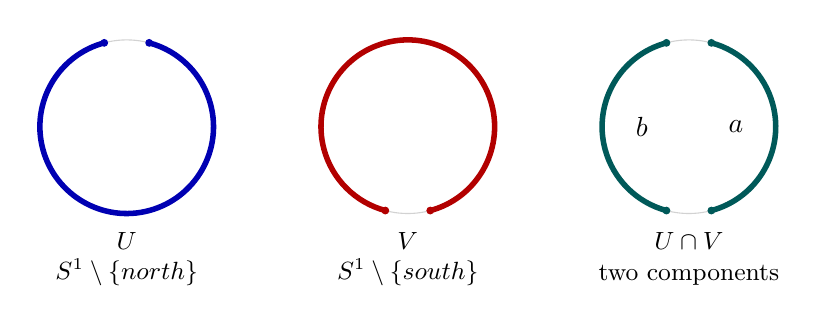
\begin{tikzpicture}[scale=1.05]
\begin{scope}[xshift=-3.4cm]
\draw[gray!35] (0,0) circle (1.05);
\draw[blue!70!black,line width=2pt] (105:1.05) arc (105:435:1.05);
\draw[fill=white,blue!70!black] (105:1.05) circle (.04) (75:1.05) circle (.04);
\node[align=center,font=\small] at (0,-1.6) {$U$\\$S^1\setminus\{\text{north}\}$};
\end{scope}
\begin{scope}
\draw[gray!35] (0,0) circle (1.05);
\draw[red!70!black,line width=2pt] (-75:1.05) arc (-75:255:1.05);
\draw[fill=white,red!70!black] (-75:1.05) circle (.04) (255:1.05) circle (.04);
\node[align=center,font=\small] at (0,-1.6) {$V$\\$S^1\setminus\{\text{south}\}$};
\end{scope}
\begin{scope}[xshift=3.4cm]
\draw[gray!35] (0,0) circle (1.05);
\draw[teal!70!black,line width=2pt] (-75:1.05) arc (-75:75:1.05);
\draw[teal!70!black,line width=2pt] (105:1.05) arc (105:255:1.05);
\foreach \a in {-75,75,105,255} \draw[fill=white,teal!70!black] (\a:1.05) circle (.04);
\node at (-.57,0) {$b$};\node at (.57,0) {$a$};
\node[align=center,font=\small] at (0,-1.6) {$U\cap V$\\two components};
\end{scope}
\end{tikzpicture}
\caption{Two punctured-circle open arcs cover $S^1$. Gaps are enlarged
schematically to show the omitted poles. Their overlap has a left and a
right component; a locally constant function chooses two independent values.}
\label{fig:mayer-vietoris-circle}
\end{figure}

\FloatBarrier

For example, cover a circle by two open arcs whose intersection has two
components, as in \cref{fig:mayer-vietoris-circle}. A locally constant
function on the overlap chooses one independent constant on each component,
so $H^0_{\mathrm{dR}}(U\cap V)\cong\R^2$. The arcs have degree-zero cohomology $\R$ and higher
cohomology zero; the intersection has degree-zero cohomology $\R^2$.
Here the arc computations follow directly from one-variable primitives.
The difference map sends $(a,b)$ to $(a-b,a-b)$. Its cokernel is one
dimensional, so the sequence recovers the one-dimensional
$H_{\mathrm{dR}}^1(S^1)$ computed directly in
\cref{thm:circle-cohomology}. The direct proof also identifies the
class by its period, whereas the sequence organizes the overlap obstruction.

\section{Singular Cohomology and de Rham's Theorem}
\label{sec:de-rham-comparison}
A singular $k$-simplex is a continuous map $\sigma:\Delta^k\to M$,
where $\Delta^k$ is the standard simplex with ordered vertices. Finite
real linear combinations form the singular chain space $C_k(M;\R)$.
The boundary is the alternating sum of restrictions to faces, with the
$i$th face given sign $(-1)^i$, starting at $i=0$. On $0$-chains the
boundary is zero. Each codimension-two
face occurs twice with opposite signs, so $\partial^2=0$.
This is a chain complex in the sense of \cref{def:chain-cochain-complex}.
Its dual spaces $C^k(M;\R)=\operatorname{Hom}(C_k(M;\R),\R)$ form
a cochain complex with $(\delta\varphi)(c)=\varphi(\partial c)$.
Their cohomology is real singular cohomology $H_{\mathrm{sing}}^k(M;\R)$.
A continuous map induces a chain map by composing simplices, and
precomposition then gives the contravariant map on cohomology.

Continuous simplices need not be differentiable, so we do not integrate
forms directly over an arbitrary continuous simplex. For a smooth simplex
(smooth on a neighborhood in its affine span), define
\[
I(\omega)(c)=\int_c\omega
=\sum_j a_j\int_{\Delta^k}\sigma_j^*\omega,
\qquad c=\sum_j a_j\sigma_j.
\]
The simplex version of Stokes, used here as part of the comparison
theorem with the same oriented-face convention, gives
\[
\int_{\partial c}\omega=\int_c d\omega,
\qquad \delta I(\omega)=I(d\omega).
\]
The first identity is understood with $c$ of dimension one larger than
the degree of $\omega$; it is the simplex version of the cubical
cancellation already verified in \cref{sec:integration-cohomology}.
Thus integration is a cochain map on smooth singular chains.
Closed forms annihilate boundaries, and exact forms annihilate cycles.
Passing from smooth to continuous singular theory and proving that this
comparison is an isomorphism are substantive parts of the following
external theorem, not consequences of Stokes alone.


\begin{theorem}[de Rham theorem; stated without proof]\label{thm:de-rham-comparison}
For every smooth manifold $M$ without boundary and $k\geq0$, there is a
natural isomorphism of real vector spaces
\[
H_{\mathrm{dR}}^k(M)\cong H_{\mathrm{sing}}^k(M;\R).
\]
\end{theorem}
The right-hand side is real singular cohomology, previewed in
Section~\ref{sec:algebraic-topology-preview}; it is defined from continuous
maps of simplices and their boundaries. The theorem says that smooth
differential forms recover that topological invariant. Naturality means
that pullback by a smooth map commutes with the isomorphisms. Integration
over smooth simplices supplies the comparison, with Stokes providing the
compatibility with boundaries. Comparing smooth and continuous chains and
proving that the resulting map is an isomorphism are substantial further
steps, not consequences of the nonzero-period tests alone. See
Lee~\cite[Theorem 18.14]{lee-smooth} and the cohomological route in
Tu~\cite[\S\S24--29]{tu-manifolds}.

\[
\boxed{\begin{gathered}
\text{An invariant built analytically from differential forms}\\
\text{agrees with a topological invariant.}
\end{gathered}}
\]
For a smooth map $f:M\to N$, naturality is the commuting square
\[
\begin{tikzcd}[column sep=large,row sep=large]
H_{\mathrm{dR}}^k(N)\arrow[r,"\cong"]\arrow[d,"f^*"'] &
H_{\mathrm{sing}}^k(N;\R)\arrow[d,"f^*"]\\
H_{\mathrm{dR}}^k(M)\arrow[r,"\cong"'] & H_{\mathrm{sing}}^k(M;\R).
\end{tikzcd}
\]
Either compare a class first and then pull it back, or pull it back first
and then compare: the result is the same.
In the language of \cref{def:natural-transformation}, these comparison
isomorphisms form a natural isomorphism between the two contravariant
cohomology functors on smooth manifolds. This is the structural meaning
of the period computations, not a new prerequisite for the main course.

\section*{Exercises}
\addcontentsline{toc}{section}{Exercises}
\begin{hexercise}{app-h-1}
Decide which of $x\,dy$, $y\,dx+x\,dy$, and $x\,dx+y\,dy$ are closed
on $\R^2$. Find primitives whenever possible and identify the obstruction otherwise.
\end{hexercise}
\begin{hexercise}{app-h-2}
Apply the operator $K$ to $dx\wedge dy$ on $\R^2$ and verify by direct
differentiation that the resulting $1$-form is a primitive. Track the signs.
\end{hexercise}
\begin{hexercise}{app-h-3}
Describe $H^0_{\mathrm{dR}}(\R\setminus\Z)$ and explain why a direct
sum over the components would give the wrong answer.
\end{hexercise}
\begin{hexercise}{app-h-4}
For an integer $m$, let $f_m:S^1\to S^1$ send the angle $t$ to $mt$.
Compute $f_m^*$ on $H^0$ and $H^1$ using the angular form and its periods.
\end{hexercise}
\begin{hexercise}{app-h-5}
On an annulus centered at the origin, prove that the angular form is
closed and not exact. Explain why every point nevertheless has a
neighborhood on which it has a primitive.
\end{hexercise}
\begin{hexercise}{app-h-6}
Use the torus period table to compute the induced map on $H^1$ for
$f(z,w)=(z^aw^b,z^cw^d)$, where $a,b,c,d\in\Z$ and the circle uses
complex multiplication. Specify which basis determines your matrix convention.
\end{hexercise}
\begin{hexercise}{app-h-7}
Give the product torus its product orientation. Show that
$\int_{T^2}\alpha_1\wedge\alpha_2=(2\pi)^2$, and conclude that this
closed $2$-form is not exact. Explain why this alone is not a computation
of the dimension of $H^2_{\mathrm{dR}}(T^2)$.
\end{hexercise}
